\section{Methodology}
\label{cost-benefit:methodology}

This Section presents a general methodology for measuring the costs and
benefits of allowing a website to access a \WAS.  We measure per-standard
benefit by using the described feature degradation technique to block page
access to the standard, manually browsing sites that use standard, and
observing the result.  We measure the per-standard cost in three ways: as a
function of the prior research identifying security or privacy issues with the
standard, the number and severity of associated historical \gls{cve}s, and the
lines of code needed to implement that standard.


\subsection{Representative Browser Selection}
\label{cost-benefit:methodology:methodology-browser}
This section describes a general methodology for evaluating the cost and
benefit of enabling a \WAS in web browsers, and then applies that
general approach to a specific browser, \textbf{\FFWithVersion}.  We use
this browser to represent modern web browsers generally for several reasons.

\textbf{First}, Firefox's implementation of \WASs is representative of how
\WASs are implemented in other popular web browsers (e.g. Chrome, Edge,
Safari).  These browsers use \gls{webidl} to define \WAPI interfaces, and
implement the underlying functionality mostly in C++, with some newer standards
implemented in \JS.  Many modern browsers even share significant amount of
code, both through shared third party libraries and by explicitly copying code
from each other's projects (for example, very large portions of Mozilla's
WebRTC implementation is taken or shared with the Chromium project in the form
of the ``webrtc'' and ``libjingle'' libraries).

\textbf{Second}, the standardized nature of the \WAPI means that measures of
\WAPI costs and benefits performed against one browser will roughly generalize
to all modern browsers; features that are frequently used in one browser will
be as popular when using any other recent browser.  Similarly, most of the
attacks documented in academic literature exploit functionality that is
operating as specified in these cross-browser standards, making it further
likely that this category of security issue will generalize to all browsers.

\textbf{Third}, using \FF allows for a direct comparison with the measurements
discussed in Chapter~\ref{measurement}, which were taken with a similar version
of \FF.  It also allows for drawing on other related research conducted on
Firefox (e.g. \cite{shin2011evaluating}).

Finally, we stress that the approach described in this Chapter would work with
any modern browser; the discussed techniques are not tied to \FFWithVersion.


\subsection{Measuring by Standard}
To measure the costs and benefits of the \WAPI, we first identified a large,
representative set browser features implemented across all modern web browsers.
We extracted the 1,392 standardized \WAPI features implemented in \FF, and
categorized those features into \NumStandards \WASs, using the same as
described in Section~\ref{measurement:data-sources:method-web-features}.

Using the features listed in the \gls{w3c}'s (and related standards
organizations) publications, we categorized \texttt{Console.prototype.log} and
\texttt{Console.prototype.timeline} with the \emph{Console API},
\texttt{SVGFilterElement.apply} and \texttt{SVGNumberList.prototype.getItem}
with the \emph{SVG} standard, and so forth, for each of the 1,392 features.
Again, this mirrors the same set of features described in
Section~\ref{measurement:data-sources:method-web-standards}.

We use these \NumStandards standards as our unit of \WAPI measurement for two
reasons.  First, focusing on \NumStandards standards leads to less of a
combinatorial explosion when testing different subsets of \WAPI functionality.
Secondly, standards are organized around high level cohesive purposes, which
are easier to convey to users who might be interested in blocking parts of the
\WAPI. However, the decision to focus on standards also came with some
drawbacks, some of which are discussed later in
Section~\ref{current-web:extension-deployment:feature-level}.


\subsection{Determining When A Website Needs A Feature}
\label{cost-benefit:methodology:manual-inspection}
This Chapter models how beneficial each \WAPI standard is by measuring
how many websites require the standard to function.  Enabling features sites do not
use provides little benefit to users.  These measurements focus on
low-trust, unauthenticated, casual browsing scenarios, and do not
attempt to capture more app-like experiences, like video chat or rich
user to user messaging.

We focus on this casual browsing scenario because it closely matches the
situations where users need to be most careful: when users first visit a new
site, and have little basis to judge the site trustworthiness.
Users can only gauge whether to trust a site with greater
capabilities once they have some familiarity with it.

Determining whether a website actually needs a feature to function is difficult.
On one end of the spectrum, when a website never uses a feature, the
site trivially does not need to feature to run correctly.  As established in
Chapter~\ref{measurement}, most features in the browser fall in this category
and are rarely used on the open web.

A website may also use a feature, but not need it to carry out a user's
goals on the site.  In many cases website will still function as desired (from
the perspective of the user), even after the site is prevented from accessing
functionality it desires.  For example, a blog may use the \textit{Canvas}
standard to invisibly fingerprint the visitor.  If a visitor's browser prevents
the site from using the \textit{Canvas} functionality, the visitor will still
be able to read the desired postings on the blog, even though the
fingerprinting attempt will fail.

This measure of ``need'' is intentionally focused on the \emph{the perspective
of the browser user}.  The usefulness of a feature to a website author is not
considered beyond the ability of the site author to deliver a user-experience
to the user. If a site's functionality is altered (e.g. tracking code is
broken, or the ability to A/B test is hampered) in a way the user cannot
perceive, then we consider this feature as not being needed from the
perspective of the browser user, and thus not needed for the site.

With this insight in mind, we developed a methodology to evaluate
whether a website needs a browser standard to function. We instructed two
undergraduate workers to visit the same website, twice in a row. Each first visit
was conducted in an unmodified \FF browser and treated as the control condition.
The worker was instructed to perform as many different actions on the page as
possible within one minute. (This is in keeping with the average dwell time a
user spends on a website, which is slightly under a minute~\cite{liu2010understanding}.)
On a news site this might mean skimming articles or watching videos, while
and on an e-commerce sites it might mean searching for products and
adding them to the cart.

The worker then visits the same site a second time.  This time, the worker's
browser is modified to disable all of the features in a \WAS, using the
technique described in Section~\ref{cost-benefit:intercepting-js}.  For another
minute, the worker attempts to perform the same actions they did during the
first visit. They then assign a score to their experience on the site:
\textbf{1} if there was no perceptible difference between the control and
treatment conditions, \textbf{2} if they noticed differences, but
were still able to complete the same tasks as during the control visit,
or \textbf{3} if they were not able to complete the same tasks as during
the control visit.

We treated a site as broken if the user could not accomplish their intended
task (i.e., the visit was coded as a \textbf{3}).  To account for the inherent
subjectivity in this approach, we had both workers test the same sites,
independently, and record their score without knowledge of the other's
experience. Our workers averaged a \PctAgreementOnStandardTests agreement
ratio. This high agreement validates that the workers were able
to consistently gauge whether \WAPI standards were necessary during
casual web browsing.


\subsection{Determining Per-Standard Benefit}
\label{cost-benefit:methodology:per-standard-benefit}
We used the above described methodology to determine the benefit of each \WAPI
standards in four steps.

First, we selected a set of websites to represent the internet as a whole.
This work considers the top 10,000 most popular websites on the Alexa rankings
as representative of the web in general, as of July 1, 2015, when this work
began.

Second, for each standard, we randomly sampled \NumSitesPerStandard sites from
the \ATK that use the standard, using the measurements from
Section~\ref{measurement}.  Where there were less than \NumSitesPerStandard
sites using the standard, we selected all using sites.  Because there are only
small differences between the \WAPI use of popular and unpopular sites, as
described in Section~\ref{measurement:results:popularity}, we made the
simplifying assumption to treat these randomly sampled \NumSitesPerStandard
sites using the standard from the \ATK as representative of all sites on the
web using the standard.

Third, we used the technique described in
Section~\ref{cost-benefit:intercepting-js} to create multiple browser
configurations, each with one standard disabled.  This yielded 75 different
browser configurations (one configuration with each standard disabled, and one
``control'' case with all standards enabled).

Fourth, we performed the manual testing described in
Section~\ref{cost-benefit:methodology:manual-inspection}.  We carried out the
above process twice for each of the \NumSitesTestedInStandardTests sites tested
for this purpose.  We carried out this process for all \NumStandards standards,
yielding the \textbf{site break rate} for each \WAS.  We define the
per-standard \textbf{site break rate} as the percentage of times the site broke
with the featured disabled, multiplied by how frequently the standard is used
in the \ATK.  We then define the benefit of a standard as a function of its
site break rate; the more sites break when a standard is disabled, the more
useful the standard is to a browser user.  The results of this measurement are
discussed in Section~\ref{cost-benefit:results}.


\subsection{Determining Per-Standard Cost}
\label{cost-benefit:methodology:per-standard-cost}
We measured the security cost of enabling a \WAS in three ways.

The first cost metric for enabling a \WAS is as a function of reported
\gls{cve}s against the standard's implementation.  Past \gls{cve}s are an
indicator of present risk for three reasons.  First, multiple past
vulnerabilities indicate that the problem domain addressed by this code that is
difficult to code securely. These code areas therefor deserve heightened
scrutiny, and carry additional risk.  Second, prior
research~\cite{ozment2006milk,zimmermann2008predicting} found that bugs fixes
introduce nearly as many bugs as they address, suggesting that code that has
been previously patched carries heightened risk for future future
vulnerabilities.  Third, recent industry practices suggest that project
maintainers asses security risk similarly; that codebases with many past
vulnerabilities should be treated with increased caution~\cite{boringssl}.

Second, we measure a \WAS~'s cost as a function of the amount of recent academic
work documenting security and privacy issues in a standard.  We searched
for attacks leveraging each \WAS in security conferences and journals between
2010 and 2015 (i.e. the five years preceding when this work was conducted).

Third, we measure a \WAS~'s cost by the number of lines of code
needed solely to implement the standard in the browser. We base this metric
on previous research that found that code complexity (measured as the
number of lines of code in function definitions) has have moderate predictive
power for discovering where future vulnerabilities will occur in the
\FF codebase~\cite{shin2011evaluating}.


\subsubsection{CVEs}
\label{cost-benefit:methodology:costs-cves}
We determined the number of \gls{cve}s previously associated with each
\WAS in three steps:

First, we searched the MITRE \gls{cve} database for all references to \FF in
\gls{cve}s issued between 2010 and 2016 resulting in \NumFirefoxCVEs \gls{cve}
records.

Second, we reviewed these \gls{cve}s and discarded \NumFirefoxCVEsOther \gls{cve}s that
were predominantly about other pieces of software, where the browser was
only incidentally related (e.g. the Adobe Flash Player
plugin~\cite{cve_2012_4171}, or vulnerabilities in web sites that are
exploitable through \FF~\cite{cve_2013_2031}).

Third, we examined each of the remaining \gls{cve}s to
determine if they documented vulnerabilities in the implementation of one of the
\NumStandards considered \WASs.  This step's goal was to exclude vulnerabilities
relating to no-\WAPI parts of the browser, such as the layout engine,
the \JS runtime, or networking libraries.
We identified \NumFirefoxStandardCVEs \gls{cve}s describing vulnerabilities in
\FF~'s implementation of \NumStandardsWithCVE standards.
\NumCVEsWithMultipleStandards \gls{cve}s document vulnerabilities in multiple
standards.

We identified which \WAS a \gls{cve} related to by reading the text
description of each \gls{cve}. We attributed \gls{cve}s to \WAS
in the following ways:

\hspace{1em}
\begin{itemize}

  \item 117 (66.9\%) \gls{cve}s explicitly named a \WAS.
  \item 32 (18.3\%) \gls{cve}s named a \JS method, structure
        or interface uniquely related to a larger standard.
  \item 21 (12\%) \gls{cve}s named a C++ class or method uniquely
        related to the implementation of \WAS, using the methodology described
        in~\ref{cost-benefit:methodology:costs-loc}.
  \item 5 (2.8\%) \gls{cve}s named browser functionality defined by a \WAS
        (e.x. several \gls{cve}s described vulnerabilities in \FF's handling of
        drag-and-drop events, which are covered by the \gls{html}
        standard~\cite{whatwg2018html}).
\end{itemize}
\hspace{1em}

We were careful to distinguish \gls{cve}s associated with \WAPI functionality
from \gls{cve}s associated with lower level functionality.  This was done to
narrowly measure the cost of \textit{only} the \WAPI implementation of the
standard.  For example, the \gls{svg} standard~\cite{svg2011standard} allows
site authors to use \JS to manipulate \gls{svg} documents embedded in websites.
We counted \gls{cve}s like \texttt{CVE-2011-2363}~\cite{cve_2011_2363} , a
``use-after-free vulnerability'' in \FF's implementation of the \JS function
for manipulating \gls{svg} documents, as part of the cost of including the
\gls{svg} \WAS in \FF.  In contrast, \gls{cve}s relating to non-\WAPI aspects
of \gls{svg} handing, were excluded from our measurements.  For example,
\texttt{CVE-2015-0818}~\cite{cve_2015_0818}, a privilege escalation bug in
\FF's \gls{svg} rendering, is not related to the \WAPI~\footnote{\gls{svg}
documents can be rendered statically, without \JS interaction.}, and so is not
counted in these measurements.


\subsubsection{Implementation Complexity}
\label{cost-benefit:methodology:costs-loc}
The third method used to evaluate the per-standard cost relates to
how much complexity does the standard bring to the code base.  To measure this,
we performed a static analysis of the \FF source to generate lower-bound
code-complexity approximations, as a count of significant lines of C/C++ code.
This measurement rests on the intuition that more complex implementations
carry greater security-costs.

This measurement considers lines of C/C++ code used \emph{only} to implement
the measured \WAS.  Lines of code shared between multiple standards are therefor
ignored in this measurement.  We call this metric as \gls{eloc}.
We compute the \gls{eloc} for each \WAS in three steps.

Step one was to build a call graph of \FF using Mozilla's DXR tool~\cite{dxr}.
DXR has two related functions. First, DXR includes a clang compiler plugin that
builds a call graph of C/C++ code bases.  Second, DXR provides tools for
querying the call graph, most significantly a web application.\footnote{An
example of the DXR interface is available at
\url{https://dxr.mozilla.org/mozilla-central/source/}.} We used this call graph
to understand how code paths related and depend on each other.  We modified DXR
to record the number of lines of code for each function.

In step two, we determined the entry points for standard in the call
graph.  Each property, method or interface defined by a \WAS has two categories
of underlying code in Firefox code, \textbf{implementation code}
(hand written code that implements \WAS's functionality), and \textbf{binding
code} (programmatically generated C++ code only called by the \JS runtime).
Binding code is generated at build time from \gls{webidl} documents. By
mapping each feature in each \gls{webidl} document to a \WAS, we are able to
associate each binding code function with a \WAS.

\begin{figure}[ht]
  \centering
  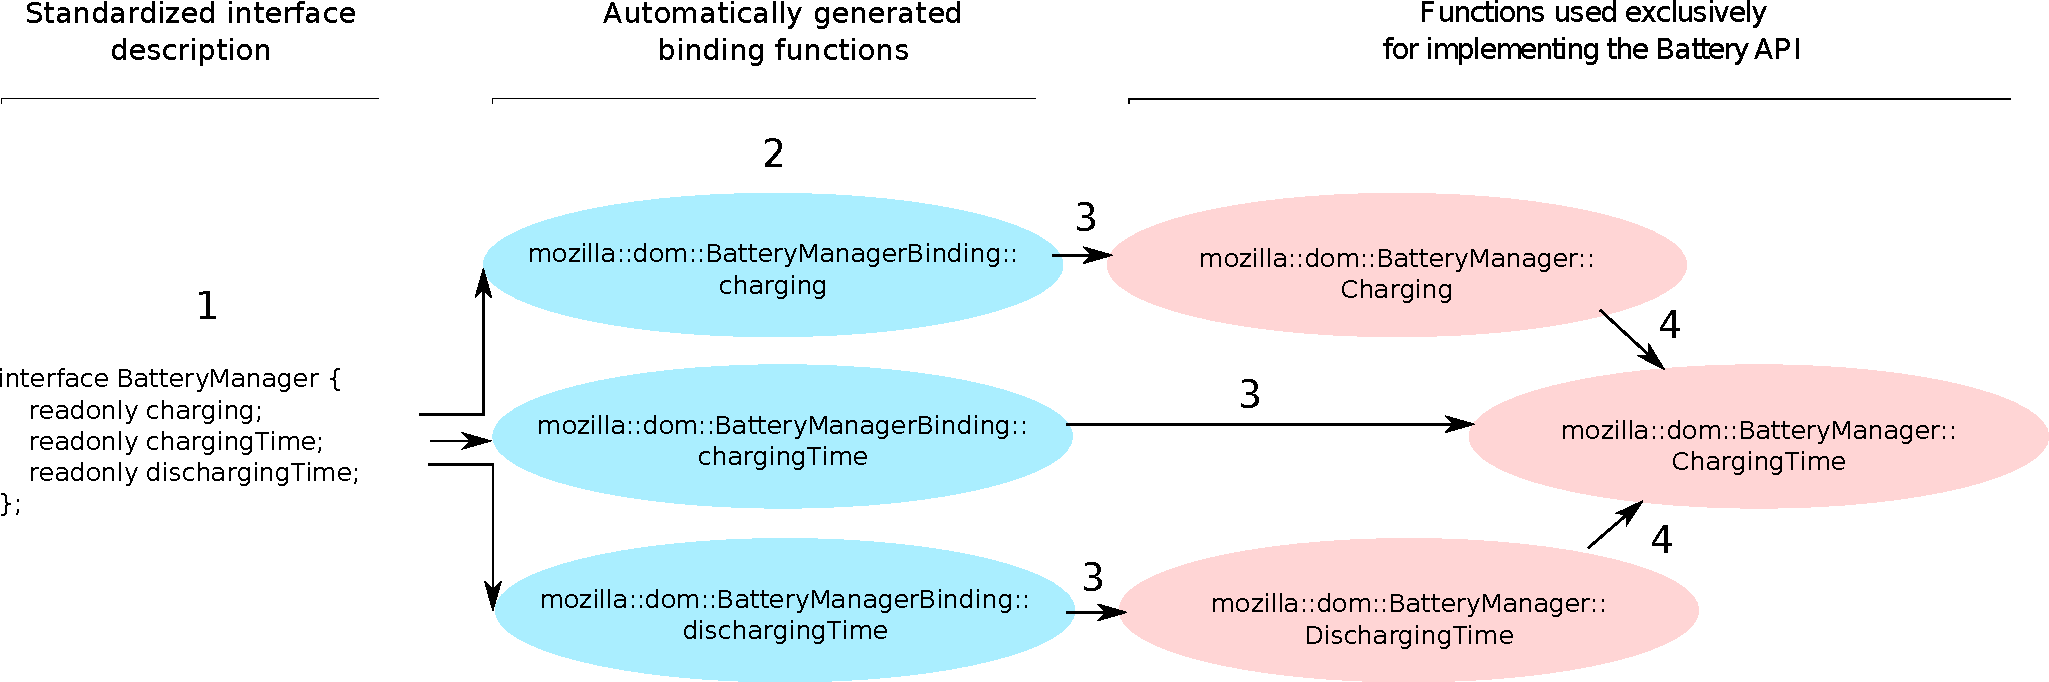
\includegraphics[width=\textwidth]{figures/prune_graph.pdf}
  \caption{An example of applying the graph pruning algorithm to a simplified version of the \textit{Battery API}.}
  \label{fig:prune-graph}
\end{figure}


Once we determined the call graph entry points for each \WAPI feature, we used
a recursive graph algorithm to identify implementation code associated with
each standard.  \ref{fig:prune-graph} illustrates this approach.  First, we
programmatically extract the standard's definitions for its binding functions,
here represented with a a simplified version of the \textit{Battery API}. Second,
we located the build-time generated binding code the \FF call graph, here
denoted by blue nodes.  Third, using the call graph, we identified which
implementation functions the binding functions call into, which are denoted by
pink nodes.  If an implementation-code (pink) node had only a single incoming edge,
we determined that this method / function was only in the code because of
the \WAS associated with those binding functions.

In the \ref{fig:prune-graph} example, algorithm begins by finding that the only
code in the \FF code base that calls the \texttt{Charging} and
\texttt{DischargingTime} methods are the binding functions generated by the
\textit{Battery API} standard.  The algorithm then marks these methods as
uniquely related to the \texttt{Battery API}.  The algorithm then repeats,
again looking for nodes with only callers from known \texttt{Battery API}
methods.  On the second iteration, the algorithm with identify the
\texttt{ChargingTime} method as solely related to the \textit{Battery API}
standard's implementation, since it is only called by functions we know to be
solely part of the \textit{Battery API}'s implementation. Thus, the lines
implementing all three of these pink implementing functions are used to compute
the \gls{eloc} metric for the \textit{Battery API}.


\subsubsection{Third Party Libraries}
\label{cost-benefit:methodology:third-party-libraries}
The above described algorithm gives a precise lower bound measurement of the
lines of code \emph{in the Firefox source} included only to implement a given
\WAS.  It does not include code from third-party libraries, which are compiled
as a separate step in the \FF build process, and thus excluded from DXR's
call-graph.

While this is a limitation of our technique, in practice it ended up bot being
significant.  In nearly all cases, third party libraries are used in multiples
places in the \FF codebase and cannot be uniquely attributed to any single
standard, and thus are not relevant to our per-standard \gls{eloc} counts.

The sole exception is the \textit{WebRTC} standard, which uniquely uses over
500k lines of third party code.  While this undercount is large, it too is
ultimately not significant to our goal of identifying high-cost, low-benefit
standards, as the high number of vulnerabilities in the standard  (as found in
\gls{cve}s) and comparatively high \gls{eloc} metric already flag the standard
as being high-cost.
